\begin{figure}
  \centering
  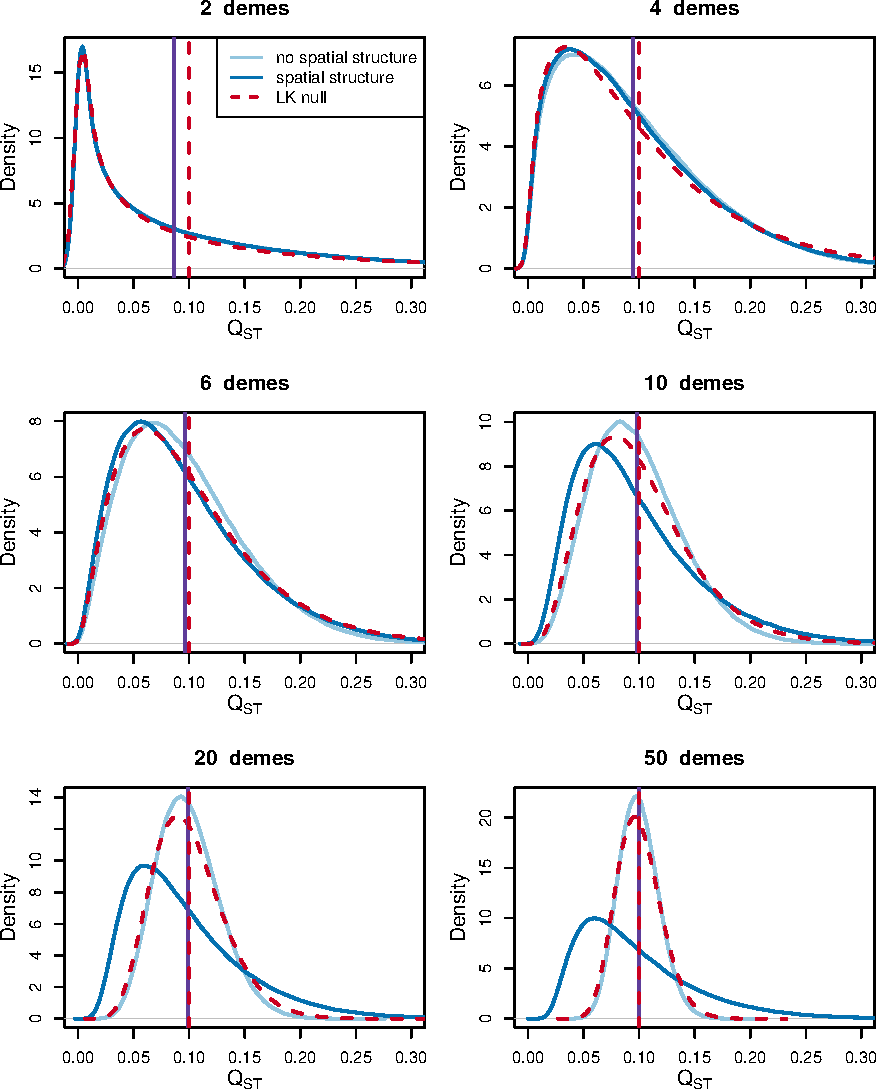
\includegraphics[width=0.8\textwidth]{qst_deme_compare.pdf}
  \caption{A comparison of the Lewontin-Krakauer (LK) distribution with the
    distribution of $Q_{ST}$ derived in this paper based on the infinitesimal
    model. A model of no spatial structure and equal migration between demes is
    compared to a stepping stone model where populations are arranged in a ring.
    $F_{ST}$ is held constant while the number of demes is increased by altering
    the migration rate.}
  \label{fig:qst_deme}
\end{figure}
\begin{figure}
  \centering
  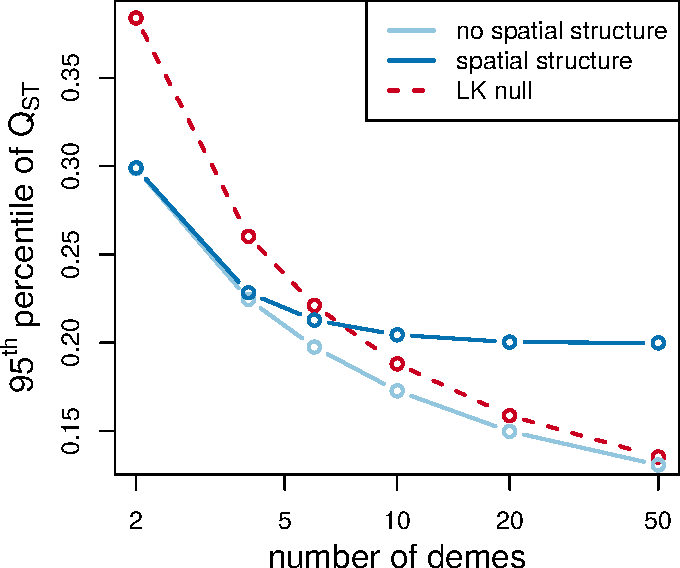
\includegraphics[width=0.5\textwidth]{qst_deme_percentile_nospace.pdf}
  \caption{Differences in the $95^{\mathrm{th}}$ percentile of the $Q_{ST}$
    distribution.}
  \label{fig:qst_perc}
\end{figure}
An important application of the neutral theory of quantitative traits is to the
divergence between groups in structured populations. A good place to start is by
asking what level of divergence is expected in the infinitesimal limit. A common
way to quantify the divergence in trait value between groups is $Q_{ST}$. This
is the variance between the group means divided by the total variance in the
population. Since this study uses a haploid model, we define
$Q_{ST} = \frac{V_{between}}{V_{between} + V_{within}}$. These variances are
defined at the population level and can be written as
\begin{equation*}
  V_{between} = \frac{1}{K} \sum_i \left( \bar{Y}_i - \bar{Y} \right)^2
\end{equation*}
and
\begin{equation*}
  V_{within} = \frac{1}{\sum_k N_k} \sum_i \sum_j \left( Y_{i,j} - \bar{Y}_i \right)^2.
\end{equation*}
Here, $Y_{i,j}$ is the trait value of individual $j$ in population $i$.

In the normal model all $Y_{i,j}$ are normally distributed. The terms
$\bar{Y}_{i} - \bar{Y}$ and $Y_{i,j} - \bar{Y}_i$ therefore are as well. When
population sizes are large, individual deviations from population means are
nearly uncorrelated as are $V_{between}$ and $V_{within}$. $V_{within}$ is
nearly constant across evolutionary realizations and is equal to
$\sum_k N_k E[\mathcal{T}_{k,k}] / \sum_k N_k$. The between group variance is more
complicated, but its distribution can be simulated from by drawing a vector of
$\bar{Y}_{i} - \bar{Y}$ values from a multivariate normal distribution with mean
zero and covariance matrix with elements
\begin{equation}
  \Cov[\bar{Y}_{i} - \bar{Y}, \bar{Y}_{j} - \bar{Y}] =
  \sigma^2(\bar{\mathcal{T}}_{i,\cdot} + \bar{\mathcal{T}}_{j,\cdot} -
  \bar{\mathcal{T}}_{\cdot,\cdot} - \bar{\mathcal{T}}_{i,j}).
\end{equation}
To simulate $Q_{ST}$ values it is not necessary to know $\sigma^2$. knowing
expected coalescent times within and between populations, perhaps measured in
units of mutations, is sufficient for simulation.

A classic result in evolutionary quantitative genetics is that $Q_{ST}=F_{ST}$
\citep{Whitlock1999}. $F_{ST}$ in this context refers to a parameter of the
population. In particular, $F_{ST} = \frac{\bar{t} - \bar{t}_0}{\bar{t}}$, where
$\bar{t}$ is the expected coalescent time for two loci sampled at random from
the entire population and $\bar{t}_0$ is the expected coalescent time for two
loci sampled within a subpopulation \citep{Slatkin1991}. This value is constant
over realizations of the evolutionary process. $Q_{ST}$ for a particular trait
could refer to a state of the population or to an estimate of this state. As
shown above, $Q_{ST}$ as a state of the population varies across evolutionary
realizations, and it does not make sense to define it as a constant parameter as
can be done for $F_{ST}$. The expectation of $V_{between}$ is
$\bar{t} - \bar{t}_0$, and the expectation of $V_{within}$ is $\bar{t}_0$.
$\frac{\E[V_{between}]}{\E[V_{between}] + \E[V_{within}]}$ is equal to $F_{ST}$,
but due to Jensen's inequality, the expectation of this ratio ($\E[Q_{ST}]$) is
actually always less than $F_{ST}$.

The null distribution of $Q_{ST}$ derived here could be useful in
goodness-of-fit tests for whether an observed value is unlikley under
neutrality. Current methods to perform such tests either compare $Q_{ST}$ either
to an empirical distribution of $F_{ST}$ values or to a $\chi^2$ distribution.
In the second case an identical distribution to that developed by
\citet{Lewontin1973} is used. This procedure was suggested by
\citet{Whitlock2009} and is implemented in the program \textit{QstFstComp}
\citep{Gilbert2015}. The Lewontin-Krakauer (LK) distribution assumes
independence between demes and provides a good approximation in populations
without spatial structure and when the number of demes is large (Figure
\ref{fig:qst_deme}). When demes are strongly correlated, such as in spatial
structured populations, the LK distribution is a very poor approximation. Even
when the distributions appear similarly shaped there are substantial differences
in tail probabilities (Figure \ref{fig:qst_perc}).

The infinitesimal model null distribution is very similar to the extension of
the Lewontin-Krakuer $F_{ST}$ test developed by \citet{Bonhomme2010} to account
for the correlation structure between subpopulations. That method treats allele
frequencies as multivariate normal with covariance matrix parameteried by
coancestry coefficients. \citet{Ovaskainen2011} use a normal model similar to
that found in the infinitesimal limit here, but the covariance matrix is also
based on coancestry coefficients. When phenotypic divergence is mostly driven by
changes in allele frequency, the coalescent and coancestry based models should
be very similar. However, the coalescent model should ultimately be preferred
since it is the correct null model at any scale of population divergence in the
infinitesimal limit. When only allele frequency data are avaiable, a coancestry
model is the only option, but it is still better to model shared ancestry
between populations than to use a single value of $F_{ST}$.
%%% Local Variables:
%%% TeX-master: "short_report.tex"
%%% End:
